\documentclass[10pt,a4paper]{article}

\usepackage[utf8]{inputenc}
\usepackage[english,russian]{babel}
\usepackage{amsmath}
\usepackage{amsfonts}
\usepackage{amssymb}
\usepackage{textcomp}
\usepackage{graphicx}
\usepackage{hyperref}
\usepackage{fancyvrb}
\usepackage{enumitem}

\usepackage[margin=17mm]{geometry}

\newcommand{\argmin}{\arg\!\min}

\begin{document}

\title{Скрытые Марковские модели переменного порядка для анализа данных
  ChIP-seq}
\author{Атаманова Анна, кафедра системного программирования СПбГУ, \url{anne.atamanova@gmail.com}}

\maketitle

\begin{abstract}
  Здесь нужно кратко описать суть работы и результаты.
  Цели работы:  
  
\makeatletter
    \AddEnumerateCounter{\asbuk}{\@asbuk}{м)}
\makeatother
\setlist{nolistsep}
\renewcommand{\labelitemi}{-}
\renewcommand{\labelenumi}{\asbuk{enumi})}
\renewcommand{\labelenumii}{\arabic{enumii})}
Целью данной работы стоит изучение марковской модели переменного порядка, ее реализация и приминение на данных Chip-seq

\end{abstract}

\section{Введение}

ДНК (дезоксирибонуклеиновая кислота) --- длинная двухцепочечная молекула, являющаяся носителем
генетической информации в биологических организмах. В клетках эукариот ДНК
находится в упакованном состоянии. Упаковка ДНК реализована с участием
специальных белковых комплексов --- нуклеосом. Химические модификации субъединиц
нуклеосомы, гистонов, могут влиять на плотность упаковки ДНК. Увеличение
плотности ДНК влияет на доступность соответствующих участков ДНК для внутренней
машинерии клетки.

%% TODO: чуть больше информации о важности изучения химических модификаций
%% хвостов гистонов

Иммунопреципитация хроматина с последующим секвенированием (chromatin
immunoprecipitation sequencing, ChIP-seq) --- это биологический протокол,
позволяющий получить информацию о наличие или отсутствии некоторой химической
модификации гистонов вдоль генома \cite{Johnson2007}. Суть метода заключается в
использовании антитела для отбора фрагментов ДНК, cвязанных с гистонами,
имеющими изучаемую химическую модификацию с последующим секвенированием. В ходе
секвенирования случайные фрагменты ДНК, читаются секвенатором в объёме,
достаточном для того, чтобы с большой вероятностью каждый фрагмент был прочитан
несколько раз. Затем для каждого полученного прочтения ищется соответствующий
ему участок последовательности генома (рис.~\ref{fig:chip-seq}). Обычно
прочтения, которым может соответствовать более одного участка в геноме,
исключают из рассмотрения.

\begin{figure}[h]
  \centering
\begin{Verbatim}[commandchars=\\\{\}]
          CAAAAGACAAATAGTGATGTCACCAATCGAGC
          --------------------------------
               GACA ATA     GTCA   AATG
              AGAC   TAGTG TGTC
               GACA   AGTG TGTCA   ATCG

          00001100001110000110000001000000
\end{Verbatim}
  \caption{Схематическое изображение выравнивания прочтений секвенатора (под чертой)
    на известную последовательность генома (над чертой).}
  \label{fig:chip-seq}
\end{figure}

Результаты эксперимента представляют в виде вектора длины генома, в котором
стоит 1, если в соответствующей позиции генома начинается хотя бы одно прочтение
и 0 в обратном случае.

%% TODO: описать разбиение на бины и ввести обозначения.

Протокол хроматин-иммунопреципитации, как и большинство биологических
протоколов, не исключает наличие в результатах эксперимента
ошибок. Недостаточная специфичность антитела, наличие ошибок секвенирования
и нестабильность положения гистонов на ДНК приводят к возникновению сигнала не
зависящего от наличия изучаемой модификации гистонов. Использование
вероятностных моделей позволяет провести анализ результатов
хроматин-иммунопреципитации с учётом наличия ошибок.

Большинство существующих моделей (TODO: ref) для данных
хроматин-иммунопреципитации основано на аппарате скрытых Марковских моделей
второго порядка с Пуассоновскими испусаниями. Использование распределения
Пуассона для покрытия, опирается на предположение о том, что в каждой
позиции генома в среднем начинается одинаковое количество прочтений. Марковский
процесс, как правило, имеет два состояния $+$ --- сигнал есть и $-$ --- сигнала
нет. Второй порядок модели означает, что состояние некоторого окна зависит только
от состояния его прямого предшественника.

Использование моделей второго порядка объясняется тем, что количество параметров
модели, а также сложность её обучения и использования экспоненциально зависят от
порядка, то есть, модель порядка $m$ требует оценки $2^m$ параметров.

%% TODO: четче объяснить привлекательность модели второго порядка и перейти к
%% цели работы.

В настоящее время, в качестве семейства искомых моделей, активное приминение находит HMM (Hidden Markov Model)\cite{Rabiner1989} второго порядка с Пуассоновским испусканием.
Данное семейство допускает предположение о том, что каждое состояние (наличие/отсутствие белка в заданной части генома) завист только от одного предыдущего.
Можно ограничиться и более лояльным допущением о том, что состояние зависит от $n$ предыдущих состояний, однако такое допущение резко увеличивает сложность модели ($O(2\textsuperscript{n})$ параметров). Также, сложность заключается в подборе этого $n$ и переобучении в случае, если не все состояния имеют одинаковые длины контекстов зависимости.
Последннее замечание подводит к идее использования VOHMM (Variable Order Hidden Markov Model)\cite{Wang2006}


\section{Скрытые марковские модели переменного порядка}

\textbf{Определение.} Последовательность случайных величин $ \{X_{i}\}_{i \in Z}$ называется \emph{цепью Маркова порядка $ m $}, если $ \forall t\in Z $

$ P(X_{t} = x_{t}|X_{t-1}=x_{t-1},X_{t-2}=x_{t-2} ... X_{-\infty}=x_{-\infty})$ = 
$ P(X_{t} = x_{t}|X_{t-1}=x_{t-1},X_{t-2}=x_{t-2} ... X_{t-m+1}=x_{t-m+1}) $ 
\\\\
\textbf{Определение.} Марковская цепь является \textit{однородной}, если вероятностное распределение преходов $P(X_{t} = x_{t}|X_{t-1}=x_{t-1},X_{t-2}=x_{t-2} ... X_{t-m+1}=x_{t-m+1})$ едино для всех $ t $.
\\
Далее будем обозначать просто $ P(x_{t}|x_{t-1}..x_{t-m+1})$
\\\\
\textbf{Определение.} \emph{Марковской моделью (Markov Model (MM)) порядка $ m $} называют вероятностную модель, описывающую однородный марковский процесс порядка $ m $.
Параметрами модели являются множество состояний $ S = \{1..n\} $ и множество переходов $ A = \{a(q, x^{m})\}_{q \in S, x^{m} \in S^{m}}$, где $a(q, x^{m}) = P(q|x^{m})$. 
\\\\
\textbf{Определение.} \emph{Скрытая Марковская модель (Hidden Markov Model(HMM)) порядка $ m $} - вероятностная модель, параметрами которой являются множество скрытых состояний $ S = \{1..n\} $, множество переходов $ A = \{a(q, x^{m})\}_{q \in S, x^{m} \in S^{m}}$ и множество распределений испусканий $ B = \{b(y,x)\}_{y \in R^{l}, x \in S}$, где $ b(y, x) = P(y|x)$. 
\\
Такая модель описывает цепь $\{Y\}_{i \in Z}$, если ее состояния были испущены из состояний марковской цепи $\{X_{i}\}_{i \in Z}$ с параметрами $ A $ согласно распределению $ P(y|x) $, и $ P(y_{t}|y_{t-1}..y_{t-m+1}) = P(x_{t}|x_{t}..x_{t-m+1})P(y_t|x_t)$  
\\\\
На рисунке (Рис \ref{ris:image}) схематично представлена скрытая марковская модель порядка 2.
\\
\begin{figure}[hbtp]
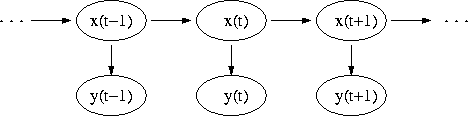
\includegraphics[scale=0.4]{img/Hmm_temporal_bayesian_net.png}
\centering
\caption{HMM order 2}
\label{ris:image}
\end{figure}
\\\\
\textbf{Определение.} \textit{Контекстное дерево} - дерево (бор), в котором каждая внутренняя вершина имеет $ n $ ребер соответствующих состояниям $ \{1..n\} $ и метку, которая является конкатенацией метки на ее родителе и метки ребра от него. Корень помечен пустой строкой. 
\\\\
\textbf{Определение.} \textit{Скрытая марковская модель переменного порядка (Variable Order Hidden Markov Model (VOHMM))}- вероятностная модель, параметрами которой являются множество скрытых состояний $ S = \{1..n\} $, конечное множество контекстов $ C=\{c_{i}\}_{i} $, где $ c_{i} $ - листья некоторого контекстного дерева, множество переходов $ A = \{a(q, c)\}_{q \in S, c \in C}$ и множество распределений испусканий $ B = \{b(y,x)\}_{y \in R^{l}, x \in S}$, где $ b(y, x) = P(y|x)$.  
\\\\\\
\textbf{Обучение модели VOHMM:}
\\
{\large Задача:} 
\\
По цепи наблюдений $ Y = (y_{1}, ... y_{T}) $ найти параметры модели $ \Lambda$, 
которые бы максимизировали правдоподобие при максимально сжатых контекстах 
\footnote{Параметр алгоритма $ \epsilon $ определяет допустимое отклонение распределений}
\\\\
{\large Алгоритм:}
\\
Параметры алгоритма: $ m $ - максимальная длина контекста, $ \epsilon $ - барьер для обрезания
\\
\begin{enumerate}
\item Инициализация контекстов.
\\
$ C_{0} = \{c| c\in S^{m}\}$
\\
Начальное распределение переходов произвольное.
\footnote{В определенных случаях (Gauss, Poisson) частотное распределение, полученное из цепи алгоритмом k-means (k=m), ускоряет работу}
\\
\item EM (Expectation–Maximization algorithm).
\\
Пересчет производится подобно алгоритму Baum-Welch для HMM
\\
Вводятся дополнительные параметры
\\
$ \alpha_{t}(c) = P(y_{1}^{t}, c(x_{t})=c| \Lambda)$
\\
$ \beta_{t}(c) = P(y_{t+1}^{T}| c(x_{t})=c, \Lambda))$
\\
$ \gamma_{t}(c) = P(x_{t}=c|Y,\Lambda) $
\\
$ \xi_{t}(q,c) = P(c(x_{t})=c, x_{t+1} = q| Y, \Lambda)$
\\
с помощью которых итеративно пересчитываются параметры модели
\\
$ \alpha_{0}(c) = p(c)b(y_{0},c)$, 
$ \alpha_{t+1}(c) = \sum_{q \in S, c'=C(cq)}{\alpha_{t}(c')a(c[0],c')b(y_{t+1},c)}$
\\
$ \beta_{T}(c) = 1$, 
$ \beta_{t}(c) = \sum_{q \in S, c'=C(qs)}{a(q,c)b(y_{t+1}, c')\beta_{t+1}(c')}$
\\
$p = P(Y|\Lambda) = \sum_{c \in C}\alpha_{T}(c)$
\\ 
$ \gamma_{t}(c) = \frac{\alpha_{t}(c)\beta_{t}(c)}{p}$
\\
$p(c) = \sum_{t}\gamma_{t}(c)$
\\
$ \xi_{t}(q,c) = \frac{\alpha_{t}(c)a(q,c)b(y_{t+1},c)\beta_{t+1}(qc)}{p} $
\\
$ a(q, c) = \frac{\sum_{t}\xi_{t}(q,c)}{p(c)}$
\\
Пересчет $ B $ зависит от принятого семейства моделей испусканий. Производится с помощью $ \gamma $ в точности также как и в алгоритме Baum-Welch.
\\
\item Обрезание дерева.
\\
Если существует внутренний лист $ s $ такой, что $ \forall q \in S \; kl(sq, s) < \epsilon $ (дети не уточняют родителя), то $ s $ становитcя листом, а все его потомки обрезаются.
\\
$kl(u, w) = \sum_{q' \in S} P(q'|u) log\frac{P(q'|u)}{P(q'|w)}$ - расстояния Кульбака-Лейблера для апостериорных распределений.
\\
\item Если на третьем шаге ничего не произошло, то алгоритм заканчивет реботу, 
иначе происходит обновление матрицы $ a $ для новых контекстов
\\
$ a(q, c) = P(q| c)$
\\
и алгоритм переходит на второй шаг.
\\
\end{enumerate}
Обозначения: 
\\
$ c(x_{t}) $ - контекст состояния $ x_{t} $ 
\\
$ C(s) $ - листья, являющиеся потомками $ s $, если $ s $ принадлежит дереву 
\\
$ C(s) $ - контекст максимальной длины, являющийся префиксом $ s $, если $ s $ не принадлежит дереву 
\\\\
\textbf{Замечание.}  Вероятностные переходы на листьях задают вероятностные переходы на всем дереве

$ p(q|s) = \frac{\sum_{c \in C(s)} {p(q|c)}}{\sum_q\sum_{c \in C(s)} {p(q|c)}} $ 
\\\\\
\textbf{Замечание.} При пересчете верятности могут очень близко подходить к нулю, что негативно сказывается на точность расчета. Для избежания этой проблемы все расчеты проходят не с вероятностями, а с логарифмми от них.
\\\\\
\textbf{Замечание.} EM может застревать в локальных максимумах функции правдоподобия.


\section{Simulation}
Проиллюстрируем работу модели на искусcтвенных данных.
\\
Из дерева \ref{ris:img_eq_Gauss_real_tree} была просэмплирована выборка размером $ T = 4000$ с Гауссовскими распределениями испусканий. Обучение проходило, начиная с контекстов длины 4. 
\\
Обученное дерево представлено на рисунке \ref{ris:img_eq_Gauss_predicted_tree}
\\
Из рисунка \ref{ris:img_eq_Gauss_plot} видно, что модель сначала 24 итерации обучалась на 16 контекстах длины 4, потом шаг обрезания сократил количество контекство до 3, и модель еще 16 итераций обучалась на них
\\
Здесь инициализация распределений переходов была равномерная. Если ее задавать с помощью алгоритма k-means, то сходимость на первом наборе контекстов будет заметно быстрее. Это видно из рисунка \ref{ris:img_Gauss}.
\footnote{Здесь можно подумать, что последние итерации лишние. Да, возможно так и есть. Барьер для остановки EM в эксперименте стоял $ 1e-2 $}
\\
Общее падение правдоподобия незначительно.
\begin{figure}[ht]\centering
	\parbox[b]{ 0.49 \textwidth}{
	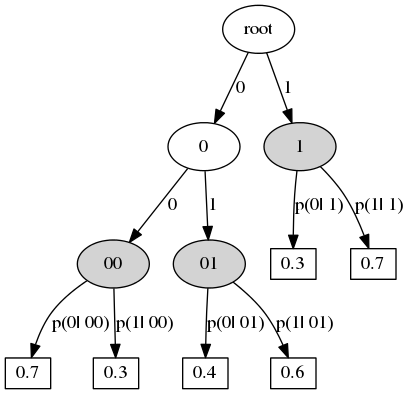
\includegraphics[scale=0.3]{img/eq_3676real_trie_.png}
	\centering
	\caption{Real tree}
	\label{ris:img_eq_Gauss_real_tree}
	
	}
\hfil \hfil%раздвигаем боксы по горизонтали
\begin{minipage}[b]{0.49 \textwidth}
	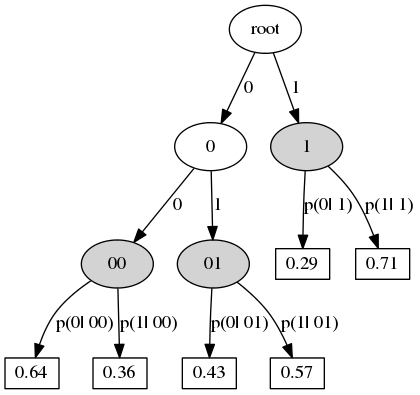
\includegraphics[scale=0.3]{img/eq_3676trie_.png}
	\centering
	\caption{Predicted tree}
	\label{ris:img_eq_Gauss_predicted_tree}
\end{minipage}
\end{figure}


\begin{figure}[hbtp]
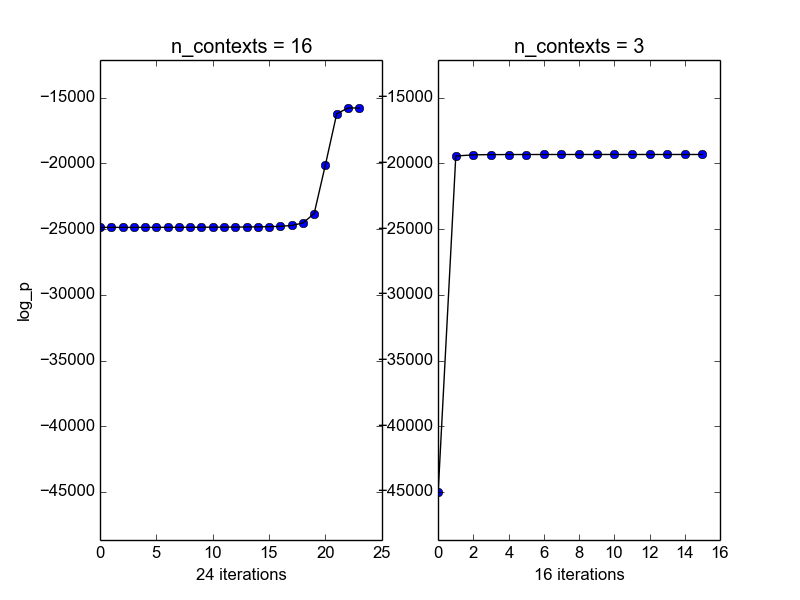
\includegraphics[scale=0.4]{img/eq_3676plot_.png}
\centering
\caption{Log likelihood}
\label{ris:img_eq_Gauss_plot}
\end{figure}


\begin{figure}[hbtp]
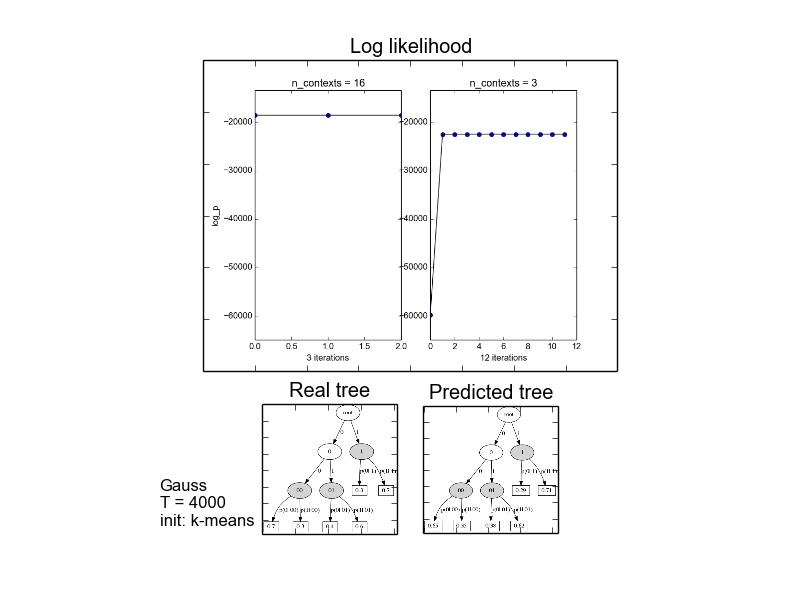
\includegraphics[scale=0.4]{img/583.jpg}
\centering
\caption{Общий график для теста с инициализацией алгоритмом k-means}
\label{ris:img_Gauss}
\end{figure}

\section{Оценка модели}

\section{Заключение}

\bibliographystyle{plain}
\bibliography{references}

\end{document}
